\documentclass[12pt]{article}   	% use "amsart" instead of "article" for AMSLaTeX format

\usepackage[a4paper,
            bindingoffset=0.2in,
            left=1in,
            right=1in,
            top=1in,
            bottom=1in,
            footskip=.25in]{geometry}
            
\usepackage[parfill]{parskip}    		% Activate to begin paragraphs with an empty line rather than an indent
\setlength{\parskip}{1ex plus 0.5ex minus 0.2ex}
\setlength{\parindent}{15pt}

\usepackage[english]{babel}
\usepackage{lipsum}
\usepackage{hyperref}                       %Uso de hipervínculos
\usepackage[labelfont=bf]{caption}          %Formato de figures
\usepackage{subcaption}                     %subfigures
\usepackage{graphicx}    
\usepackage{amssymb}
\usepackage{amsmath}
\usepackage[style = ieee]{biblatex}          %Manejo de bibliografía



\usepackage{listings}
\usepackage{xcolor}

\definecolor{codegray}{gray}{0.9}
\definecolor{darkgreen}{rgb}{0,0.5,0}
\definecolor{darkblue}{rgb}{0,0,0.5}

\lstdefinelanguage{VHDL}{
  morekeywords=[1]{library, use, entity, is, port, in, out, end, architecture, of, begin, signal, process, if, then, else, elsif, when, others},
  morekeywords=[2]{std_logic, std_logic_vector},
  sensitive=true,
  morecomment=[l]--,
  morestring=[b]",
}

\lstset{
  language=VHDL,
  keywordstyle=[1]\color{blue}\bfseries,
  keywordstyle=[2]\color{darkgreen},
  commentstyle=\color{gray}\ttfamily,
  stringstyle=\color{darkblue},
  basicstyle=\ttfamily\small,
  numbers=left,
  numberstyle=\tiny,
  stepnumber=1,
  numbersep=5pt,
  captionpos=b,
  breaklines=true,
  breakatwhitespace=false,
  tabsize=2,
  showstringspaces=false
}


\usepackage{graphicx}
\usepackage{amssymb}

\addbibresource{references.bib}



\title{FPGA laboratory report}
\author{Diego Figueroa -- 2485776}
\date{\today}							% Activate to display a given date or no date

\begin{document}
\maketitle


\section{Convolutional encoder}

The goal of this practice is to implement a convolutional encoder, of a specific code of rate $R=1/2$, with memory $m=2$, and polynomials generators $g_0(x) = x^2+1$ and $g_1(x)=x^2+x+1$. This specific convolutional encoder can be represented by a shift register and some xor operations, as seen in figure \ref{fig:conv_code_sh_reg}, or as a finite state machine as seen in figure \ref{fig:conv_code_fsm}.

\begin{figure}[htb]
    \centering
    \begin{subfigure}[t]{0.5\textwidth}
        \centering
        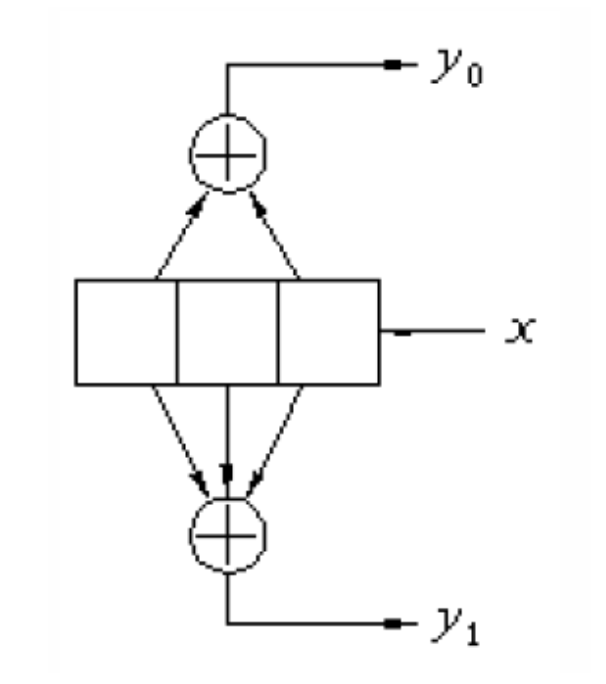
\includegraphics[height=0.7\textwidth]{img/conv_code_sh_reg}
        \caption{Representation as shift register}
        \label{fig:conv_code_sh_reg}
    \end{subfigure}%
    \begin{subfigure}[t]{0.5\textwidth}
        \centering
        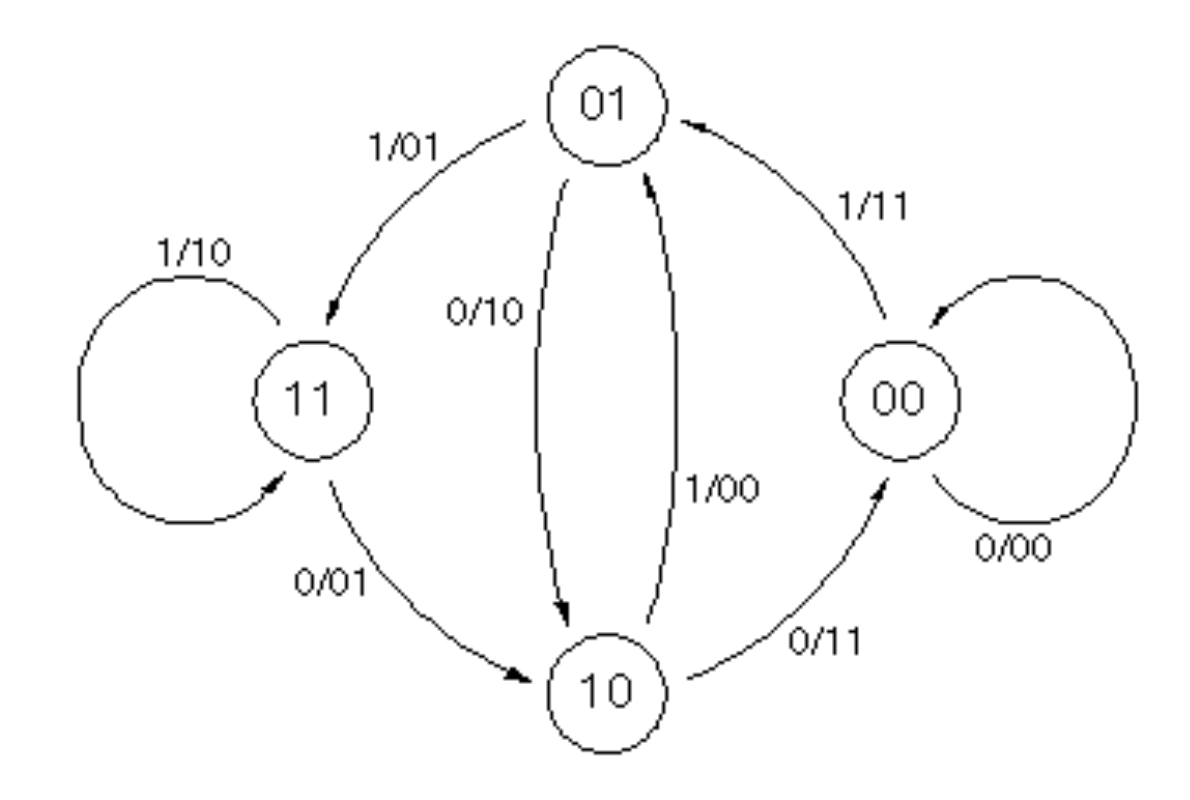
\includegraphics[height=0.7\textwidth]{img/conv_code_fsm}
        \caption{Representation as a finite state machine}
        \label{fig:conv_code_fsm}
    \end{subfigure}
    \caption{Caption place holder}
    \label{fig:conv_code_reps}
\end{figure}




\subsection{Symbol schematic implementation}

To implement this encoder in the FPGA, the first Method used was to use the schematic interface of Quartus II. For this propose the representation of a shift register of the convolutional encoder is well suited, so it is implemented as seen in figure \ref{fig:conv_code_sch}. There the shift register is done with 3 D-flipflops conected in series, with a common clock and reset, and no preset is used. Finally the two output bits are generated with xor gates using the signals stored in the registers.

Finally the circuit is simulated, and the results can be seen in section \ref{sec:conv_code_results}.


\subsection{VHDL implementation}
For VHDL the representation of the code as a FSM is used. The code describing this machine can be seen listing \ref{code:conv_code_vhdl} in the Annex, this code is based in an example of a state machine in \cite{vhdl_douglas}.

In the architecture declaration, the first thing done is defining a new enum type to store the states of the state machine, then some signals are defined. Two processes are used, one for the state logic i.e. describing the outputs and what transitions are done in each state; and the other to update the state and read the incoming data on every rising edge of the clock.

Finally the circuit is simulated, and the results can be seen in section \ref{sec:conv_code_results}.



\subsection{AHDL implementation}
For the AHDL implementation a FSM is also used. The code in this case can be seen in listing \ref{code:conv_code_ahdl}, and is inspired by the example found in \cite{ahdl}.

The first three lines correspond to the declaration of the component, then two variables are declared, one of type \lstinline{MACHINE}, where the states are declared, and one of type \lstinline{node}. In the description of the behavior, the clock and the reset of the state machine ara assigned, \lstinline{d_in} is implemented as a D-flipflop to store the incoming data over a clock period, and the behavior of the FSM is described as a table.

It is important to notice that the state machine is implemented with asynchronous outputs, that means that while being in one state, the outputs can change if the inputs change, even before the clock edge. That is why it is important the flip flop for \lstinline{d_in}, so it has a stable value over a clock period.

Finally the circuit is simulated, and the results can be seen in section \ref{sec:conv_code_results}.


\subsection{Simulation results}
\label{sec:conv_code_results}

In figure \ref{fig:sim_conv_code} can be seen the simulations result of the encoders, the first two signals (from top to bottom) are the clock and a reference clock with a phase difference to change the data. The third signal is the input binary data, the forth signal is the reset signal.

\begin{figure}[htbp]
\begin{center}
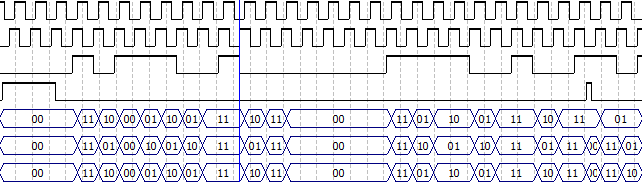
\includegraphics[width=\textwidth]{img/conv_code_comp_sim}
\caption{Simulation results of the three convolutional codes encoders.}
\label{fig:sim_conv_code}
\end{center}
\end{figure}


Finally we see the signals of the tree encoders: AHDL, VHDL and Schematic implementation. The first part of the data is de binary representation of 0x$B9$, and then there is some random data. It is evident that the three encoders have the same output which is also the expected one given the desired code. The only difference is at the end of the simulation when the reset signal goes to one for a small time. Here the two last encoders behave the same, but the first is different, this is because the AHDL implementation has a synchronous reset while the other two have an asynchronous reset.




\section{Running light}
The goal of this practice is to familiarize with the FPGA board, its built elements, such as leds push buttons, switches and seven segments displays, and program the FPGA to test the results of a circuit in real life

\subsection{Functional description}
The circuit has a series of functional requirements:
\begin{itemize}
\item Using the leds of the board, make a running light that goes from left to right and back, by turning off the current led and turning on the next one in a line, so it seems like a moving light (it is important to take into account the speed of the moving light, so it is possible to perceive the effect with the eyes).
\item Use the seven segments to count how many times the light has gone from one side to the other.
\item Add the possibility to change the speed of the running light with the use of some switches.
\item Add de ability of giving a desired pattern that moves through the leds, by using the switches.
\item Change the operation mode of the circuit between \textbf{Start}, \textbf{Stop}, \textbf{Reset, Load pattern}, by using the push buttons.
\item Change the direction of the lights between \textbf{left}, \textbf{right} or \textbf{for- and backward}
\end{itemize}

\subsection{Digital Design and VHDL implementation}
To accomplish the functional specifications of the circuit, the design is broken into smaller pieces, which are then interconnected in a top level entity. Each of the subsystems and the top level entity are describen next.


\subsubsection{lr\_ring\_reg}
To accomplish the moving pattern in both directions the entity \lstinline{lr_ring_reg} is used. It is a shift register that shift all the values to the left (in a circular manner) on every rising edge of the clock. It also has a \lstinline{pattern_in} signal that is hard set in the registers if the signal \lstinline{load} is set to high. Finally the output is a pattern moving left, and other moving right, which is implemented simply by reversing the order of the ring register.

The implementation  in VHDL can be seen in listing \ref{code:lr_ring_reg}. In line 7 a generic is defined to specify the number of cells in the ring register. In the architecture some intermediate signals are defined. Then in line 16 - 19 a concurrent generate statement is used to define \lstinline{pattern_out_l} as simply \lstinline{pattern_out}, and \lstinline{pattern_out_r} as the reversed version of \lstinline{pattern_out}. A process is used to do the shift operation, and an other process is used to load a pattern and update \lstinline{pattern_out}.

\subsubsection{clk\_div\_n}
A clock divider is needed for different proposes: first to make the effect of the moving light visible, but also to change the speed of the light. Also a clock that is $n_\text{led}$ (number of leds) slower than the clock used for the ring register is useful to signal when a light has done a full run from one side to the other (which is needed to count the runs of the light).

For this reason an entity for a clock divider is defined, which can change the division number during operation. The code for this module is in listing \ref{code:clk_div_n}. In the entity declaration a generic is used to define the counter width. The only process of the architecture resets the counter \lstinline{cnt} and the pulse to 0 if \lstinline{rst} is 1. Otherwise on a \lstinline{clk_in} rising edge if \lstinline{n} changes, set \lstinline{cnt} to 1 and \lstinline{pulse_reg} to 0, if \lstinline{cnt = n - 1}, \lstinline{cnt} is set again to 0 and \lstinline{pulse_reg} to 1, otherwise \lstinline{cnt} is increased by one and \lstinline{pulse_reg} set to 0. The result is a small positive pulse every \lstinline{n} pulses of \lstinline{clk_in}.

\subsubsection{decimal\_cnt}

This module is used to count the number of runs of the light. It is based on the module \lstinline{digint_cnt}, and is just a series connection of $n$ \lstinline{decimal_cnt}'s, as can be seen in listing \ref{code:decimal_cnt}. And \lstinline{digint_cnt} just counts on every \lstinline{inc} rising edge, and if gets to 9 it goes back to 0 and generate a pulse on \lstinline{inc_out} (see code on listing \ref{code:digit_cnt}).

\subsubsection{seven\_segments}
This module is really simple, it just outputs the needed signals for a seven segments display depending on the given number it receives, it is just implemented as a look up table in a concurrent statement as seen in listing \ref{code:seven_segments}.


\subsubsection{speed\_rom}
To change the speed of the light a ROM is implemented, where different values of $n$ are stored and used as inputs of \lstinline{clk_div_n}, this file is automatically generated using a python code (see listing \ref{code:create_speed_rom}) depending in some parameters, an example the VHDL rom can be seen in listing \ref{code:speed_rom}.

\subsubsection{const\_types\_pkg}
A package to define some types and constants is also used to improve the readability of the code in \lstinline{running_light} (see code in listing \ref{code:const_types_pkg}).

\subsubsection{running\_light}

Finally the top level entity is described in listing \ref{code:running_light}. A structural schematic of the model can be seen in figure \ref{}. And the different modules are controlled using the FSM seen in figure \ref{}. In general the fast clock of the FPGA is divided by \lstinline{speed}, this clock goes to the \lstinline{lr_ring_reg}, and is also divided to count the number of runs whit the module \lstinline{decimal_cnt}. The signal going to the leds is taken from a multiplexer depending on the current value \lstinline{dir}, and with the FSM the circuits switches between the modes \textbf{Start}, \textbf{Stop}, \textbf{Reset, Load pattern}.


%%% TO DO:
% a lot of images and FIR filters.


\section{FIR filters}


\subsection{Low pass}



\subsection{High pass}



\subsection{Band pass}



\subsection{Band stop}



\subsection{Project with the 4 filters}


\printbibliography


\section*{Annex}

\lstinputlisting[caption={Code in VHDL for the FSM of the convolutional code encoder.}, label={code:conv_code_vhdl}]{../convolutional_code_VHDL/convolutional_code_VHDL.vhd}

\lstinputlisting[caption={Code in VHDL for the FSM of the convolutional code encoder.}, label={code:conv_code_ahdl}, firstline=4]{../convolutional_code_AHDL/convolutional_code_AHDL.tdf}

\lstinputlisting[caption={Code in VHDL for \lstinline{lr_ring_reg}.}, label={code:lr_ring_reg}]{../running_light/lr_ring_reg.vhd}

\lstinputlisting[caption={Code in VHDL for \lstinline{clk_div_n}.}, label={code:clk_div_n}]{../running_light/clk_div_n.vhd}

\lstinputlisting[caption={Code in VHDL for \lstinline{decimal_cnt}.}, label={code:decimal_cnt}]{../running_light/decimal_cnt.vhd}

\lstinputlisting[caption={Code in VHDL for \lstinline{digit_cnt}.}, label={code:digit_cnt}]{../running_light/digit_cnt.vhd}

\lstinputlisting[caption={Code in VHDL for \lstinline{seven_segments}.}, label={code:seven_segments}]{../running_light/seven_segments.vhd}

\lstinputlisting[caption={Code in python for creating the speed room.}, label={code:create_speed_rom}, language=python]{../running_light/create_speed_rom.py}

\lstinputlisting[caption={Code in VHDL for \lstinline{speed_rom}.}, label={code:speed_rom}]{../running_light/speed_rom.vhd}

\lstinputlisting[caption={Code in VHDL for \lstinline{const_types_pkg}.}, label={code:const_types_pkg}]{../running_light/const_types_pkg.vhd}

\lstinputlisting[caption={Code in VHDL for \lstinline{running_light}.}, label={code:running_light}]{../running_light/running_light.vhd}







\end{document}  